\chapter{Grundlagen}
\label{ch:grundlagen}

\section{Design Smells}
\label{sec:grundlagen-design-smells}

Design Smells bezeichnen strukturelle Probleme in einem Softwaresystem, die die Qualität des Systems negativ beeinflussen~\citep{software_design_smell_detection}. Sie führen nicht unbedingt zu Fehlern beim Übersetzen oder Ausführen des Systems. Das bedeutet, dass ein System trotz Design Smells korrekt funktionieren kann. Jedoch erschweren Design Smells das Verstehen, Testen, Erweitern und Warten des Systems~\citep{software_design_smell_detection}. Daher dienen sie als Hinweise auf Wartbarkeitsprobleme und zeigen, an welchen Stellen ein Refactoring oder Reengineering sinnvoll sein kann. Design Smells können auf verschiedenen Ebenen auftreten. Manche betreffen nur einzelne Codeabschnitte, beispielsweise eine zu lange Methode. Andere betreffen die Architektur des Systems und damit mehrere Komponenten gleichzeitig. Solche Smells werden als \textit{Architektur-Smells} bezeichnet und wirken sich auf das Gesamtsystem aus~\citep{refactoring_for_software_architecture_smells}. In verteilten Legacy-Systemen entstehen Architektur-Smells häufig dadurch, wie Services miteinander kommunizieren und wie sie redundant betrieben werden. Beispiele dafür sind \textit{synchrone Request-Response-Ketten}~\citep{tiwari_unveiling_2024, liebig_2025_architectural_refactoring} und \textit{heterogene Redundanzmodi}~\citep{choudhary_rajesh_high_2025, liebig_2025_architectural_refactoring}. \textit{Architektur-Smells} liegen nicht in einem einzelnen Codeabschnitt, sondern verteilen sich über die Kommunikationspfade, Abhängigkeiten und Betriebsmodi mehrerer Services. Daher reicht ein lokales Code-Refactoring oft nicht aus. Stattdessen kann ein Reengineering auf Architekturebene notwendig sein. Aus diesem Grund werden im nächsten Abschnitt die Begriffe \textit{Reengineering} und \textit{Refactoring} voneinander abgegrenzt.

\section{Reengineering und Refactoring}
\label{sec:grundlagen-reengineering-refactoring}

\textit{Refactoring} bezeichnet die Umstrukturierung von bestehendem Code, bei der die interne Struktur verbessert wird, ohne das externe Verhalten des Systems zu verändern~\citep{laguna_systematic_2013}. Neben diesem \textit{Code-Refactoring} gibt es \textit{Architectural Refactoring}, das statt einzelner Codeabschnitte die Architektur eines Systems betrifft, beispielsweise Kommunikationspfade oder Betriebsmodi. \textit{Reengineering} ist weiter gefasst und bezeichnet die Untersuchung und Veränderung eines bestehenden Systems, um es in eine neue Form zu überführen~\citep{laguna_systematic_2013}. Es ist besonders für Legacy-Systeme relevant, die weiterhin betrieben werden, aber nur schwer oder mit hohem Risiko geändert werden können~\citep{stevens_systems_1998}. In dieser Masterarbeit wird ein \textit{Architektur-Reengineering} betrachtet. Dabei wird nicht der Code des Legacy-Systems geändert, sondern die Art, wie die Komponenten des Systems miteinander interagieren. Dadurch werden die Auswirkungen der Design Smells reduziert, ohne die bestehende Funktionalität zu verändern.

\section{Legacy Proxy System}
\label{sec:grundlagen-lps}

\gls{lps} ist ein \textit{Architektur-Reengineering-Ansatz} für verteilte Legacy-Systeme. Dabei wird eine \textit{Proxy-Schicht} zwischen den bestehenden Services des Legacy-Systems eingefügt, die deren synchrone Kommunikation über einen Message Broker in eine asynchrone Kommunikation überführt. Dadurch werden Design Smells wie \textit{synchrone Request-Response-Ketten} reduziert, ohne den Quellcode der Services zu ändern. Die Architektur und die Komponenten von \gls{lps} werden im Abschnitt~\ref{sec:lps} im Detail beschrieben.

\section{Asynchrone Messaging-Protokolle}
\label{sec:grundlagen-messaging-protocolls}

Asynchrone Messaging-Protokolle bilden die Grundlage sowohl des bestehenden \gls{lps} als auch des in dieser Masterarbeit entwickelten \gls{alps}. Sie ermögli\-chen eine räumliche und zeitliche Entkopplung von verteilten Systemkomponenten. Anstatt Services über synchrone, blockierende Aufrufe wie \gls{http} miteinander zu verbinden, wird die Kommunikation über einen Message Broker geleitet~\citep{hohpe2004enterprise}.

\subsection{Message Queuing Telemetry Transport}
\label{sub:grundlagen-mqtt}

\gls{mqtt} ist ein leichtgewichtiges Protokoll, das ursprünglich für Umgebungen mit eingeschränkter Bandbreite und instabilen Netzwerken entwickelt wurde~\citep{thangavel2014performance}. \gls{lps} verwendet die Protokollversion \gls{mqtt}~5.0. Diese erweitert frühere Versionen unter anderem um ein verbessertes Session-Management und detaillierte Fehlercodes~\citep{oasis2019mqtt, hivemq_mqtt5_essentials}. Die Kommunikation folgt einer \textit{Client-Broker-Architektur}~\footnote{Clients kommunizieren nie direkt miteinander, sondern ausschließlich über den Broker. Dadurch sind sie räumlich voneinander entkoppelt~\citep{eugster2003many}.}~\citep{oasis2019mqtt}. Das Routing der Nachrichten basiert auf einer hierarchischen \textit{Topic-Struktur}: \textit{Publisher} senden Nachrichten an \textit{Topics}, und \textit{Subscriber} abonnieren die \textit{Topics}, deren Nachrichten sie empfangen möchten~\citep{oasis2019mqtt, eugster2003many}. Ein zentrales Merkmal von \gls{mqtt} sind die \gls{qos}-Stufen, die das Zustellverhalten von Nachrichten festlegen~\citep{oasis2019mqtt}. Eine \gls{qos}-Stufe gilt dabei jeweils nur für die Übertragung zwischen zwei direkt verbundenen Teilnehmern, also zwischen \textit{Publisher} und Broker bzw.~zwischen Broker und \textit{Subscriber}. Die Spezifikation unterscheidet drei Stufen, die jeweils einen unterschiedlichen Kompromiss zwischen Protokoll-Overhead und Zuverlässigkeit darstellen.

\subsubsection{QoS~0 (At-Most-Once)}

Bei \gls{qos}~0 wird eine Nachricht ohne Bestätigung nach dem \textit{Best-Effort}-Prinzip zugestellt. Der Sender speichert die Nachricht nicht und überträgt sie auch nicht erneut. Ob die Nachricht ankommt, hängt somit ausschließlich von der zugrunde liegenden \gls{tcp}-Verbindung ab. Da keine Bestätigungen ausgetauscht werden, besitzt \gls{qos}~0 den geringsten Proto\-koll-Overhead und die geringste Latenz~\citep{oasis2019mqtt, hivemq_mqtt5_essentials}.

\subsubsection{QoS~1 (At-Least-Once)}

Bei \gls{qos}~1 wird garantiert, dass eine Nachricht mindestens einmal zugestellt wird. Der Sender speichert die Nachricht so lange, bis der Empfänger den Erhalt mit einem \texttt{PUBACK}-Paket bestätigt. Bleibt diese Bestätigung aus, wird die Nachricht erneut übertragen. Geht jedoch nicht die Nachricht selbst, sondern nur das \texttt{PUBACK}-Paket verloren, erhält der Empfänger dieselbe Nachricht mehrfach. Dadurch können Duplikate entstehen~\citep{oasis2019mqtt}. Abbildung~\ref{fig:mqtt-qos-1} zeigt neben dem Normalbetrieb das Verhalten bei einem solchen Paketverlust. Da die Bestätigung ausbleibt, überträgt der Publisher die Nachricht erneut, wodurch beim Broker ein Duplikat entsteht.

\begin{figure}[H]
    \centering
    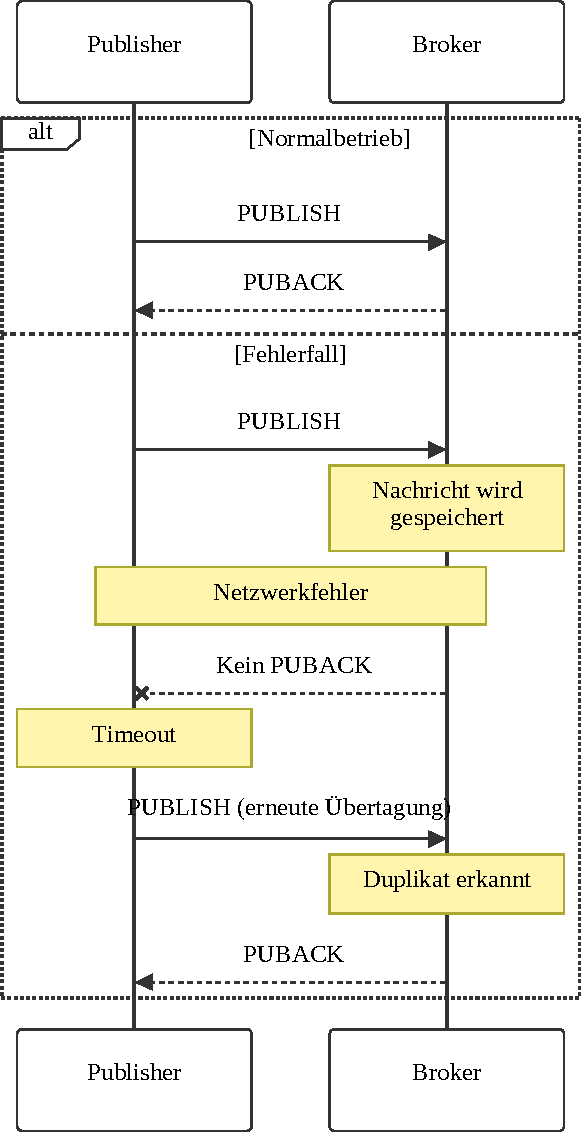
\includegraphics[width=0.4\textwidth]{./img/mermaid/mqtt_qos_1.pdf}
    \caption{Nachrichtenfluss unter \gls{qos}~1 mit möglicher Duplikatbildung bei ausbleibendem \texttt{PUBACK}.}
    \label{fig:mqtt-qos-1}
\end{figure}

\subsubsection{QoS~2 (Exactly-Once)}

\gls{qos}~2 ist die höchste Stufe und garantiert, dass eine Nachricht genau einmal zugestellt wird. Dafür wird ein zweiphasiger Handshake aus insgesamt vier Paketen verwendet. Zunächst sendet der Sender das \texttt{PUBLISH}-Paket, dessen Erhalt der Empfänger mit dem \texttt{PUBREC}-Paket bestätigt. Danach sendet der Sender ein \texttt{PUBREL}-Paket, das der Empfänger abschließend mit \texttt{PUBCOMP}-Paket bestätigt~\citep{oasis2019mqtt}. Bis zum Empfang vom \texttt{PUBREL}-Paket speichert der Empfänger die Paket-\gls{id} der Nachricht. Wird dieselbe Nachricht aufgrund eines Netzwerkfehlers erneut übertragen, erkennt der Empfänger sie anhand der gespeicherten Paket-\gls{id} als bereits empfangen. Durch diesen zusätzlichen Koordinationsaufwand steigen jedoch sowohl das übertragene Datenvolumen als auch die Latenz deutlich an~\citep{thangavel2014performance}. Abbildung~\ref{fig:mqtt-qos-2} zeigt den Ablauf dieses Handshakes.

\begin{figure}[H]
    \centering
    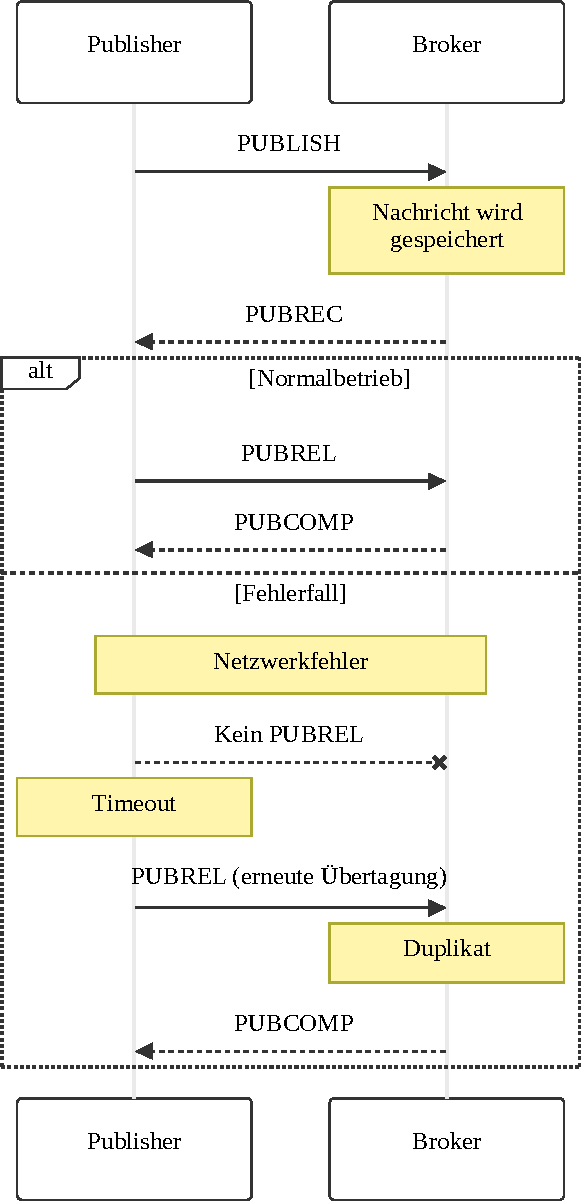
\includegraphics[width=0.4\textwidth]{./img/mermaid/mqtt_qos_2.pdf}
    \caption{Vierstufiger Handshake unter \gls{qos}~2 zur Duplikatvermeidung.}
    \label{fig:mqtt-qos-2}
\end{figure}

\subsubsection{Shared Topics}


\subsection{Advanced Message Queuing Protocol}
\label{sub:grundlagen-amqp}

Während \gls{mqtt} ursprünglich für ressourcenbeschränkte Umgebungen entwickelt wurde~\citep{thangavel2014performance}, ist \gls{amqp} ein Protokoll für den zuverlässigen Nachrichtenaustausch in Enterprise-Systemen~\citep{vinoski2006advanced, ohara2007toward}. Von \gls{amqp} existieren zwei Versionen, die sich grundlegend unterscheiden. Version~1.0 ist ein OASIS-Standard und legt nur fest, wie Nachrichten zwischen zwei Teilnehmern übertragen werden~\citep{oasis2012amqp10}. Version~0-9-1 definiert zusätzlich ein Modell für den internen Aufbau des Brokers~\citep{amqp091}. Der in dieser Masterarbeit verwendete Broker \textit{RabbitMQ}~\citep{rabbitmq_broker} basiert auf Version~0-9-1. Daher beziehen sich die folgenden Abschnitte auf diese Version.

\subsubsection{Komponentenmodell}

Bei \gls{mqtt} senden Publisher ihre Nachrichten direkt an Topics. \gls{amqp} verwendet dagegen ein Modell aus vier Komponenten: \textit{Producer}, \textit{Exchange}, \textit{Queue} und \textit{Consumer}~\citep{amqp091}. Ein Producer sendet Nachrichten nie direkt an eine Queue, sondern immer an einen Exchange. Der Exchange ist eine Routing-Komponente innerhalb des Brokers. Er entscheidet anhand von Regeln, an welche Queues eine Nachricht weitergeleitet wird. Diese Regeln werden als Bindings bezeichnet. Eine Queue speichert die Nachrichten so lange, bis ein Consumer sie konsumiert~\citep{amqp091, hohpe2004enterprise}. Abbildung~\ref{fig:amqp_topology} zeigt dieses Modell anhand einer typischen Broker-Topologie.

\begin{figure}[H]
    \centering
    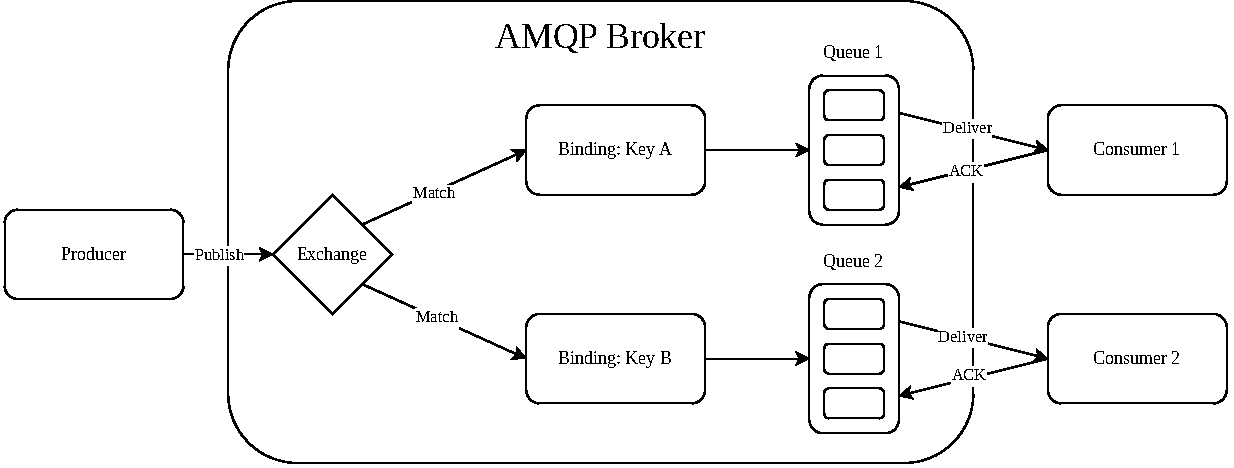
\includegraphics[width=0.95\textwidth]{./img/drawio/amqp_topo.pdf}
    \caption{Komponentenmodell und Routingpfad einer typischen \acrshort{amqp}-basierten Broker-Topologie.}
    \label{fig:amqp_topology}
\end{figure}

\subsubsection{Exchange-Typen}

Das Routing zwischen Exchange und Queue basiert auf zwei Schlüsseln. Den \textit{Routing Key}, der vom Producer an die Nachricht angehängt wird, und den \textit{Binding Key}, der festgelegt wird, wenn eine Queue an einen \textit{Exchange} gebunden wird. Wie die beiden Schlüssel miteinander verglichen werden, hängt vom Typ des \textit{Exchanges} ab. Die wichtigsten Typen sind~\citep{amqp091}:

\begin{itemize}
    \item \textbf{Direct Exchange}~\citep{rabbitmq_exchange_direct}: Eine Nachricht wird nur an die Queues weitergeleitet, deren Binding Key genau dem Routing Key der Nachricht entspricht. Dadurch lassen sich Nachrichten gezielt an bestimmte Consumer verteilen~\citep{rabbitmq_tut_work_queues, eip_competing_consumers}.

    \item \textbf{Fanout Exchange}~\citep{rabbitmq_exchange_fanout}: Der Routing Key wird ignoriert. Jede Nachricht wird in alle Queues kopiert, die an den Exchange gebunden sind. Dadurch lässt sich eine One-to-Many-Kommunikation einfach umsetzen~\citep{rabbitmq_tut_pubsub}.

    \item \textbf{Topic Exchange}~\citep{rabbitmq_exchange_topic}: Der Routing Key besteht aus Wörtern, die durch Punkte getrennt sind, z.\,B.~\texttt{regions.na.cities.boston}. Binding Keys können Wildcards enthalten: \texttt{*} steht für genau ein Wort und \texttt{\#} für null oder mehrere Wörter.
\end{itemize}

\subsubsection{Bestätigungen und Flusskontrolle}

Damit keine Nachrichten verloren gehen, werden die sogenannten \textit{Consumer-\gls{ack}} verwendet. Der Broker löscht eine Nachricht erst dann aus der Queue, wenn der Consumer ihre erfolgreiche Verarbeitung mit einem \gls{amqp}-\gls{ack} bestätigt. Kann der Consumer eine Nachricht nicht verarbeiten, sendet er ein \gls{amqp}-\gls{nack}~\citep{rabbitmq_confirms}. Ist dabei der Parameter \texttt{requeue = true} gesetzt, legt der Broker die Nachricht zurück in die Queue, damit sie erneut zugestellt werden kann~\citep{rabbitmq_confirms}. Bricht die Verbindung zum Consumer ab, bevor er eine Nachricht bestätigt hat, legt der Broker diese Nachricht automatisch zurück in die Queue~\citep{amqp091}. Der Parameter \texttt{prefetch\_count} steuert zusätzlich die Flusskontrolle. Er legt fest, wie viele unbestätigte Nachrichten ein Consumer gleichzeitig vom Broker erhalten darf. Ein \texttt{prefetch\_count} von~1 erzwingt eine \textit{Stop-and-Wait-Semantik}\footnote{Stop-and-Wait-Semantik bezeichnet ein Kommunikationsverfahren, bei dem der Sender nach dem Versand einer Nachricht wartet und erst nach Erhalt einer expliziten Bestätigung die nächste Nachricht übermittelt~\citep{tanenbaum2011computer}.}: Der Broker liefert die nächste Nachricht erst aus, wenn die vorherige bestätigt wurde.

\subsubsection{Reihenfolge und Partitionierung}

\gls{amqp} garantiert die Reihenfolge von Nachrichten nur unter engen Bedingungen. Die Nachrichten müssen über denselben Kanal\footnote{Ein Kanal (\textit{Channel}) ist eine leichtgewichtige, virtuelle Verbindung, von der mehrere über eine einzige \gls{tcp}-Verbindung zum Broker gemultiplext werden~\citep{amqp091}.} gesendet, über denselben Pfad in dieselbe Queue geleitet und von einem einzigen Consumer nacheinander verarbeitet werden~\citep{amqp091}. Verarbeiten mehrere Consumer dieselbe Queue parallel, kann die Reihenfolge verloren gehen. Für Systeme, die eine geordnete Verarbeitung pro Entität brauchen und gleichzeitig anhand von mehreren Consumern horizontal skalieren sollen, reicht das nicht aus. Eine Lösung dafür ist das Konzept der \textit{Partitioned Logs}. Dabei werden Nachrichten anhand eines Schlüssels immer derselben Partition zugeordnet. Dadurch bleibt die Reihenfolge pro Schlüssel erhalten~\citep{kleppmann2017designing}. In dieser Masterarbeit wird dieses Konzept mit zwei Erweiterungen von \textit{RabbitMQ} umgesetzt, die über den \gls{amqp}-Standard hinausgehen:

\begin{itemize}
    \item \textbf{Consistent-Hash-Routing (\texttt{x-consistent-hash})}: Ein spezieller Ex\-change-Typ, der den Hashwert des Routing Keys berechnet und die Nachricht anhand dieses Werts einer von mehreren Queues zuordnet~\citep{rabbitmq_consistent_hash_exchange}. Solange sich die Menge der gebundenen Queues nicht ändert, landen alle Nachrichten mit demselben Routing Key in derselben Queue.

    \item \textbf{Single Active Consumer (\texttt{x-single-active-consumer})}: Eine Eigenschaft einer Queue, die sicherstellt, dass immer nur ein einziger Consumer Nachrichten aus dieser Queue erhält, auch wenn mehrere Consumer registriert sind~\citep{cogoluegnes2022rabbitmq}. Fällt dieser Consumer aus, übernimmt ein anderer registrierter Consumer.
\end{itemize}

Die Implementierung von \gls{alps} ist zwar auf \textit{RabbitMQ} zugeschnitten, sind die verwendeten Konzepte jedoch nicht auf \textit{RabbitMQ} beschränkt. Andere Message Broker bieten vergleichbare Funktionen an. Dadurch wird ein starker \textit{Vendor-Lock-in}\footnote{Vendor-Lock-in bezeichnet die starke technische Abhängigkeit von einem konkreten Anbieter oder Produkt.} vermieden. So unterstützt beispielsweise \textit{LavinMQ}~\citep{lavinmq_broker} ebenfalls \textit{Consistent-Hash-Routing}~\citep{lavinmq_consistent_hash} und \textit{Single Active Consumer}~\citep{lavinmq_single_active_consumer}. \textit{Apache ActiveMQ Artemis}~\citep{artemis_broker} bietet mit \textit{Message Grouping}~\citep{artemis_message_grouping} eine vergleichbare Funktion zum \textit{Consistent-Hash-Routing} und setzt das Prinzip des \textit{Single Active Consumers} mit \textit{Exclusive Queues}~\citep{artemis_exclusive_queues} um.

\section{Erlang}
\label{sec:grundlagen-erlang}

... \textit{coming soon}
